\chapter{Design of Tests}

% Describe the way we plan on performing our
% tests and why it'll kick everyone's asses
% --------- No pseudocode needed -----------
No application is complete until it has been tested
as thoroughly as possible for security holes, broken
functionality, and any other lacking features.
Shipping without testing is a guarantee to have
all manner of bugs and security holes. However, even
with thorough testing, it is not usually possible to
find and resolve every flaw before shipment. To this end,
developers utilize \emph{testing suites} to try and
test programs efficiently and effectively. Tests can be
designed for individual units and components as well as
the broader system and the integration of the units.
While not perfect for finding all flaws in a program
(usually errors are discovered by looking
for them, which generally requires either knowledge of an
existing error or ``luck'' in an error making itself
apparent during development), testing can serve to find
almost all errors and flaws in an application.

However, developers face a dilemma. Developing an
evolving application can cause existing tests to
become outdated, while designing and running tests
is time taken away from actually building the application.

A modern approach to this tradeoff is to build the
feature set of an application around measurable,
predefined tests \cite{wiki:tdd}. In this technique,
known as Test-driven Development, developers iteratively
define tests for intended future features, confirm that those
features are not yet implemented (by running those tests),
and then implementing the solutions. Though this approach
does not (generally) test for all possible interplay
between components, it is usually employed in high-paced
development environments such as ours, where the coverage provided is
usually respectable enough to prevent most problems.

Accordingly, we first define the features and tests we
plan on developing around, proceed to analyze the coverage
offered by these tests, and then briefly discuss how we
intend to test the integration of the components.

% list and describe the test cases that will
% be programmed and used for unit testing
\section{Test Cases}

Due to project constraints, we cannot afford to thoroughly
test existing packages for functionality we incorporated to
streamline the design process. These packages include Ruby
on Rails
as well as Ruby gems (packages) for interfacing with Yahoo! Finance,
various databases (ie MySQL, SQLite), the Resque queueing system,
and other auxilliary package for Rails. Likewise, we
cannot unit test
the HTTP server we are using (Apache) and its Ruby 
extension (Phusion Passenger) or any of the databases. Rather
we will focus on testing just the units of our application and
their integration with each other.

% Discuss checking the routing, ie that all routes and permissions
% are enforced
\subsection{Routing}

As described earlier, Capital Games contains models for
users, managers, administrators, trades, etc. Intrinsic to the Rails web framework
we employ, most of these models are represented internally to the 
controller as ``resources'' \cite{guides:routing}. At any
point in time, any user (even a non-user!) could attempt to gain
access to a resource to which they are not privileged, such as an
administrator panel. Routing unit tests will confirm that only
authorized users will be able to access restricted pages. As an
extension of this premise, Routing unit tests will also confirm
that pages with low privileges are accessible to all users and
front-facing pages can be seen even without being logged in.

% Discuss that Rails does autmoatic validation but we have to test
% this anyway since it's so important
\subsection{Database Models}

Because of the data-centric design of Capital Games, protecting 
the integrity of the database entries is of the utmost importance. 
The Ruby on Rails framework has safeguards and validation for this 
purpose, but we still need to thoroughly unit test each of the 
models to ensure that only permissible combinations of attributes 
are able to be entered, and that proper error handling occurs to 
resolve attempts at improper attribute definition.

\subsection{Queueing System}

Capital Games heavily relies upon the queueing system to act as a 
computational highway for all asynchronous tasks.  Due to the 
nature of this system we must prepare for race conditions; the 
different ways our data can be effected based upon the order of 
executing processes that are acting upon the queue. We will need 
to prepare a set of tests to express how the queue performs when 
open orders are altered by other processes during different phases 
of the queueing system. Based on our test results it might be 
necessary to implement data locking.

\subsection{Finance Adapter}

Whenever using external resources it is vital to understand the 
different ways in which they communicate not just when functioning 
as expected, but also when failing to perform properly.  Since we 
do not have the ability to shut down the external Financial 
Adapter's Servers we can not run tests that give us feedback on 
what functionality to expect on failure.  This leaves us without 
the ability to test the Financial Adapter and instead pro-actively 
safeguard against failure. Due to this we must build a wrapper that 
anticipates all perceivable failures coming from the Financial Adapter.

% Describe the test coverage
\section{Test Coverage}

In order to attain full functionality of Capital Games without bugs, 
we must be sure that none of its parts have errors themselves.  Due 
to many dependencies such as other running processes, system states, 
and transitions, the same test will need to be preformed for each 
possible configuration to make sure that each part works in every 
possible scenario that it can be ran. This will require extending 
certain tests to run at the same time as background processes, and 
having parts called from all possible initiating parts. When working 
with integrated parts it is not simply enough to assume that parts 
will work once integrated just because they work independently. By 
extensively testing each possible run case we ensure that there are 
no points of failure once the system is launched.


% Describe integration testing strategy
\section{Integration Testing}

In order to achieve the most thorough testing, Capital Games will be 
tested using the bottom-up strategy. Each part of Capital Games that 
we wrote will be extensively tested individually first. However 
simply testing each part individually is not enough due to race 
conditions and other integration issues that may exist in the 
systems described above. Because of this, parts must be tested after 
integration as well.  Knowing that functionality is state specific 
and transition specific for any state machine, each test must also be 
ran in all possible states. In addition to all previously listed 
conditions, tests need to be preformed at different times to make sure 
that functionality during backend asynchronous tasks do not have any 
bugs. We have chosen the bottom-up testing strategy based on the 
principle that bugs at the bottom level will dictate bugs at the 
top level, while bugs at the top level may very well be independent 
of bottom level performance. By carefully analyzing every part to part 
integration we can work our way up to a flawless design.

\section{Test Cases}

\begin{figure}[b]
\centering
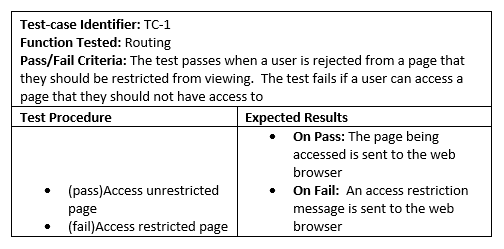
\includegraphics[width=5in]{./Diagrams/TestCases/tc1.png}
\caption{ Test Case 1.}
\end{figure}

\begin{figure}[b]
\centering
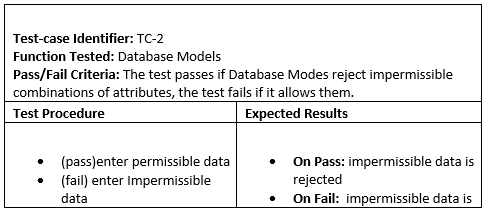
\includegraphics[width=5in]{./Diagrams/TestCases/tc2.png}
\caption{ Test Case 2.}
\end{figure}

\begin{figure}[b]
\centering
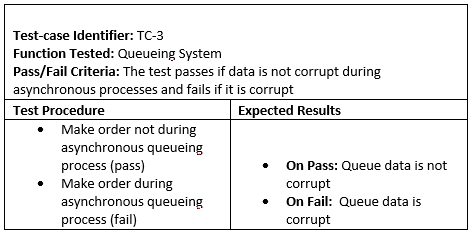
\includegraphics[width=5in]{./Diagrams/TestCases/tc3.png}
\caption{ Test Case 3.}
\end{figure}

\begin{figure}[b]
\centering
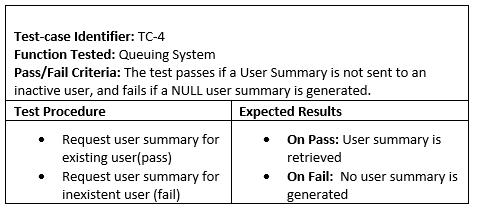
\includegraphics[width=5in]{./Diagrams/TestCases/tc4.png}
\caption{ Test Case 4.}
\end{figure}